\documentclass[11pt,letterpaper]{article}
\usepackage[margin=0.88in,headheight=15pt]{geometry}
\usepackage[T1]{fontenc}
\usepackage[utf8]{inputenc}
\usepackage{lmodern,microtype}
\usepackage{amsmath,amssymb,amsthm,mathtools}
\usepackage{booktabs,tabularx,array,longtable}
\usepackage{tikz}
\usetikzlibrary{positioning,arrows.meta,calc,fit,shapes.geometric}
\usepackage{fancyhdr,xcolor}
\usepackage[hyphens]{url}
\usepackage{xurl}
\usepackage[backend=biber,style=numeric,sorting=none,maxbibnames=8,giveninits=true]{biblatex}
\addbibresource{references.bib}
\setcounter{biburlnumpenalty}{100}
\setcounter{biburlucpenalty}{100}
\setcounter{biburllcpenalty}{100}
\AtBeginBibliography{\small\raggedright}
\setcounter{tocdepth}{1}
\definecolor{ink}{HTML}{163346}
\definecolor{teal}{HTML}{176A70}
\definecolor{pale}{HTML}{EDF4F5}
\definecolor{muted}{HTML}{52616B}
\usepackage[colorlinks=true,linkcolor=teal,citecolor=teal,urlcolor=teal,pdfauthor={P versus NP Research Program},pdftitle={Signed Four-Port Equality--Balance Networks},pdfsubject={Model specification and canonical certified contraction framework}]{hyperref}
\pagestyle{fancy}
\fancyhf{}
\fancyhead[L]{\small\sffamily\color{muted} STRICT-EB4-v1}
\fancyhead[R]{\small\sffamily\color{muted} Research specification}
\fancyfoot[L]{\small\sffamily\color{muted} Version 1.0 \enspace|\enspace 27 November 2026}
\fancyfoot[R]{\small\thepage}
\renewcommand{\headrulewidth}{0.4pt}
\renewcommand{\footrulewidth}{0pt}
\setlength{\parindent}{0pt}
\setlength{\parskip}{0.55em}
\setlength{\emergencystretch}{3em}
\renewcommand{\arraystretch}{1.17}
\newtheorem{theorem}{Theorem}[section]
\newtheorem{lemma}[theorem]{Lemma}
\newtheorem{proposition}[theorem]{Proposition}
\newtheorem{corollary}[theorem]{Corollary}
\theoremstyle{definition}
\newtheorem{definition}[theorem]{Definition}
\newtheorem{example}[theorem]{Example}
\newtheorem{obligation}[theorem]{Open obligation}
\newcommand{\EB}{\ensuremath{\mathsf{EB}_4}}
\newcommand{\SAT}{\ensuremath{\mathsf{SAT}}}
\newcommand{\UNSAT}{\ensuremath{\mathsf{UNSAT}}}
\newcommand{\UNK}{\ensuremath{\mathsf{UNKNOWN}}}
\newcommand{\bits}{\{0,1\}}
\newcommand{\Ftwo}{\mathbb F_2}
\newcommand{\Sol}{\operatorname{Sol}}
\newcommand{\NAE}{\operatorname{NAE}}
\newcommand{\sha}{\operatorname{SHA256}}
\newcommand{\abs}[1]{\lvert#1\rvert}
\newcolumntype{Y}{>{\raggedright\arraybackslash}X}
\newcolumntype{L}[1]{>{\raggedright\arraybackslash}p{#1}}
\newcommand{\status}[1]{\textsf{\small\textbf{#1}}}
\newcommand{\id}[1]{\nolinkurl{#1}}
\tikzset{process/.style={draw=teal,fill=pale,rounded corners=3pt,align=center,minimum height=9mm,text width=43mm,font=\small},arrow/.style={-{Latex[length=2.2mm]},thick,draw=muted},port/.style={circle,draw=ink,fill=white,minimum size=5.5mm,inner sep=0pt,font=\small},core/.style={circle,draw=ink,fill=pale,minimum size=11mm,font=\large\bfseries}}
\begin{document}
\thispagestyle{empty}
{\small\sffamily\bfseries\color{teal} MATHEMATICAL MODEL AND RESEARCH PROTOCOL}\par
\vspace{0.45em}
{\color{ink}\LARGE\bfseries Signed Four-Port Equality--Balance Networks\par}
\vspace{0.35em}
{\large Canonical normalization, cooperative certificates, and the universal aggregate-contraction problem\par}
\vspace{0.65em}
{\sffamily\small P versus NP Research Program\hfill Version 1.0 \enspace|\enspace 27 November 2026\par}
\vspace{0.7em}
\noindent\colorbox{pale}{\parbox{\dimexpr\linewidth-2\fboxsep\relax}{\small\textbf{Mathematical status.} The strict signed E4/B4 feasibility language is NP-complete by an explicit reduction. Exact equality normalization and the restricted terminals specified below are sound. The existence of a uniformly discoverable, polynomially bounded aggregate contraction on every unresolved input is \textbf{open}. This manuscript is a technical specification and proof framework, not a claimed resolution of P versus NP.}}
\section*{Abstract}
We define a Boolean constraint model on a finite simple four-regular graph. Every vertex has four ordered ports, each carrying a bit. An equality vertex requires all four bits to coincide; a balance vertex requires exactly two of them to be one. Each edge transmits its bit either unchanged or complemented. A constructive reduction from 3-SAT shows that feasibility is NP-complete even without free constants, dangling ports, or parallel edges. We give a canonical, source-indexed quotient that eliminates all signed equalities, retains exact integer balance and enables affine, matching, bounded-interface and other verified operations. The research objective is a uniform deterministic procedure that either decides feasibility or strictly decreases a polynomially bounded potential on the entire unresolved state, including every guarded obligation and all charged resource costs. Parallel proof tracks operate on identical content-addressed inputs, exchange checkable deductions and combine only compatible guarded certificates. We specify the semantic and resource contracts, the shared instance registry, and the precise universal progress obligation that remains to be established.\par
{\small\textbf{Keywords:} Boolean constraint satisfaction; signed graphs; exact balance; NP-completeness; certified contraction; proof DAGs; aggregate work; content-addressed instances.}
\vspace{0.55em}
\clearpage
{\small\tableofcontents}
\vspace{0.5em}

\section{Scope and mathematical objective}\label{sec:scope}
The program selects one NP-complete decision language, strict signed four-port equality--balance feasibility, as the common target for algorithmic and lower-bound research. The notation \(\EB\) denotes this language; E4 and B4 denote its two allowed local vertex signatures. The authoritative repository model is RT01 \cite{rt01}, and the common research assignment, compiler and certificate protocol are pinned in \cite{ebdirective,compiler,identifiers}.

The central objective is to determine whether every unresolved network admits a polynomially discoverable, sound contraction or an exact terminal decision, with a polynomial \emph{aggregate} progress bound. The objective is neutral with respect to \(\mathrm P=\mathrm{NP}\) and \(\mathrm P\ne\mathrm{NP}\). Successful termination on a restricted family is evidence for a module, not a universal solver. Failure of a specified module is a scoped obstruction, not a time lower bound for arbitrary computation.

The term \emph{canonical approach} has three distinct meanings in this document: a deterministic syntactic equality quotient, a shared procedure for certified progress, and an exact byte-level identity convention for cooperative work. None is a claim that arbitrary residuals can be canonically identified up to semantic equivalence, graph isomorphism, or satisfiability at polynomial cost. Sections~\ref{sec:quotient}--\ref{sec:protocol} give an implementable baseline and formal contracts; the universal coverage theorem in Section~\ref{sec:potential} remains an open obligation.

\section{The strict signed E/B model}\label{sec:model}
\subsection{Input, ports and local signatures}
\begin{definition}[Strict input]
A valid instance is a tuple
\[
 I=(V,P,\tau,\mathcal E),\qquad
 V=\{0,\ldots,v-1\},\qquad P=V\times\{0,1,2,3\},
\]
where \(\tau:V\to\{E,B\}\) gives the type of each vertex and \(\mathcal E\) is a perfect pairing of the ports with signs. Write an edge as \((p,q,s)\), with \(s\in\bits\). The graph on the vertex owners of the ports must be simple and undirected: no edge joins a vertex to itself, and no unordered pair of vertices owns two edges. Each port is used exactly once. Consequently \(\abs P=4v\) and \(\abs{\mathcal E}=2v\).
\end{definition}
Each port \(p\) has an independent Boolean variable \(x_p\) before constraints are imposed. With \(x_{i,j}=x_{(i,j)}\), the allowed local relations are
\begin{align}
 E_4&=\{(0,0,0,0),(1,1,1,1)\},\label{eq:e4}\\
 B_4&=\{a\in\bits^4:\textstyle\sum_{j=0}^{3}a_j=2\}.\label{eq:b4}
\end{align}
The B4 relation has precisely six legal words. Its sum is over the integers, not over \(\Ftwo\). Every edge imposes
\begin{equation}\label{eq:edge}
 x_p\oplus x_q=s,
\end{equation}
where \(\oplus\) denotes addition in \(\Ftwo\). A sign of zero means equality and a sign of one means complementarity. An E vertex acts as a synchronization junction; a B vertex acts as an exact two-of-four occupancy constraint.

\begin{figure}[htbp]
\centering
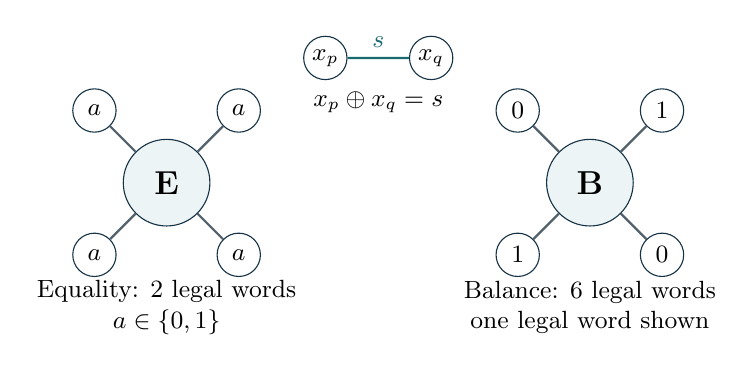
\begin{tikzpicture}[scale=0.96]
 \node[core] (e) at (0,0) {E};
 \node[core] (b) at (5.6,0) {B};
 \foreach \ang in {45,135,225,315}{\node[port] (ep\ang) at (\ang:1.35) {$a$};\draw[thick,muted] (e)--(ep\ang);}
 \foreach \ang/\val in {45/1,135/0,225/1,315/0}{\node[port] (bp\ang) at ($(b)+(\ang:1.35)$) {\val};\draw[thick,muted] (b)--(bp\ang);}
 \node[align=center,font=\small] at (0,-1.65) {Equality: 2 legal words\\$a\in\bits$};
 \node[align=center,font=\small] at (5.6,-1.65) {Balance: 6 legal words\\one legal word shown};
 \node[port] (p) at (2.1,1.65) {$x_p$};\node[port] (q) at (3.5,1.65) {$x_q$};
 \draw[thick,teal] (p)--node[above,font=\small] {$s$}(q);
 \node[font=\small] at (2.8,1.06) {$x_p\oplus x_q=s$};
\end{tikzpicture}
\caption{The two vertex signatures and signed transport. The displayed ports are schematic; in a valid original network every port belongs to exactly one edge.}
\label{fig:signatures}
\end{figure}

\subsection{Feasibility, encoding and model boundaries}
Let \(F_I(x)\) be the conjunction of all vertex relations and edge constraints. The decision problem is
\[
 \EB=\{\operatorname{enc}(I): I\text{ valid and }\exists x\in\bits^{4v}\ F_I(x)\}.
\]
A witness is an assignment to all original ports, checked by evaluating every original vertex and edge. Invalid encodings may be rejected at parsing. A negative certificate is a checkable argument that no assignment exists; neither a solver timeout nor absence of a witness is such an argument.

For the shared benchmarks the encoding is ASCII JSON with a final LF, using the exact property order \id{format}, \id{types}, \id{edges}. The format field is \id{STRICT-EB4-v1}; vertex IDs are zero-based positions in \id{types}, port IDs are \(4i+j\), and edge IDs are zero-based positions in \id{edges}. Each edge record is the ordered triple of endpoint port IDs and sign. Let \(N\) be the bit length of the original encoded byte stream. All resource bounds in this paper are stated in \(N\), including all index widths, source reads and representation changes. Equivalent explicitly indexed encodings are polynomially interconvertible; they need not have the same fingerprint.

The original graph has no auxiliary unary pins, dangling ports, degree-two vertices or parallel edges. Such objects may occur in a verified \emph{residual representation}, with exact semantics and provenance, but do not change the original promise. There is no assumption of planarity, geometric embeddability, shared-wheel structure, bipartiteness, or bounded treewidth. A theorem for a stricter subclass requires a separate reduction or structural argument.

\subsection{Complement symmetry and parity}
\begin{lemma}[Gauge symmetry]\label{lem:gauge}
Complementing all port bits in a connected component preserves all original constraints. On an unguarded connected component with at least one port, fixing one chosen port to zero preserves the existence of a solution.
\end{lemma}
\begin{proof}
Equality is invariant under complementation, and B4 remains legal because \(4-2=2\). The XOR of two complemented bits is unchanged. A solution with the selected port equal to one can therefore be complemented within that component to give a solution with the port equal to zero. The selected port is not thereby proved logically forced in the original unguarded network. Under a guard, the normalization is permitted only when the guard is invariant or a correct guarded equivalence is proved.
\end{proof}
A simple necessary condition follows by summing all port bits modulo two. At every E vertex the sum is even, and at every B vertex the sum is exactly two. Each edge contributes its sign to the sum, hence in each connected component
\begin{equation}\label{eq:parityglobal}
 \bigoplus_{e\in\mathcal E_C}s_e=0
\end{equation}
is necessary for feasibility. A component with odd total sign is immediately infeasible. Even total sign is not sufficient for a general mixed network.

\section{NP-completeness of the model}\label{sec:npc}
The following reconstruction of RT01 \cite{rt01,rt01code} makes the model assumptions and witness maps explicit. We use the classical NP-completeness of satisfiability with at most three literals per clause \cite{karp1972}.
\begin{theorem}[Strict signed E4/B4 feasibility is NP-complete]\label{thm:npc}
There is a uniform polynomial-time many-one reduction from 3-SAT to \(\EB\). The constructed graph is simple, undirected, four-regular, and uses only E4 and B4 vertices and signed edges. For each source assignment, a network witness decoding to it exists if and only if the assignment satisfies the source formula.
\end{theorem}
\begin{proof}
Membership in NP follows from the explicit port witness and polynomial-time verifier.

\textbf{Step 1: relative literal encoding.} For each occurring Boolean source variable \(u\), introduce a carrier \(X_u\). Introduce one common anchor carrier \(f\). Decode the source bit as \(u=X_u\oplus f\). For a literal \(\ell\) on \(u\), its physical value is \(L=X_u\oplus\epsilon_\ell\), where \(\epsilon_\ell=0\) for a positive literal and 1 for a negative literal. The literal truth value is \(L\oplus f\). A clause with physical literals \(A,B,C\) is satisfied exactly when \(A,B,C,f\) are not all equal. Clauses of size one or two are padded by repeating a literal; an empty clause is handled by two opposite repeated-literal unit clauses on a fresh variable. This preserves feasibility.

\textbf{Step 2: split the four-input not-all-equal relation.} For a fresh bit \(z\),
\begin{equation}\label{eq:nae}
 \NAE_4(A,B,C,f)\quad\Longleftrightarrow\quad
 \exists z\; \NAE_3(A,B,z)\land\NAE_3(1-z,C,f).
\end{equation}
If \(A=B\), the first condition forces \(z=1-A\); otherwise it allows both values. If \(C=f\), the second condition forces \(z=C\); otherwise it allows both values. The forced choices conflict precisely when \(A=B=C=f\). This establishes both directions and supplies a constructive selection of \(z\).

\textbf{Step 3: implement each NAE triple by exact balance.} For bits \(a,b,c\),
\begin{equation}\label{eq:slack}
 \NAE_3(a,b,c)\quad\Longleftrightarrow\quad
 \exists d\in\bits:\ a+b+c+d=2.
\end{equation}
For a legal triple, the uniquely determined slack is \(d=2-(a+b+c)\). A constant triple would require \(d=2\) or \(d=-1\), neither of which is a bit. Thus a clause uses two B4 nodes, with separate slacks and shared clause carrier \(z\).

\textbf{Step 4: synchronize repeated carriers.} Duplicate each B4 node, with both copies sharing the same carriers, literal signs and slack. This preserves exact projected feasibility and makes the number \(d\) of occurrences of each carrier even. For \(d\ge4\), use a path of \(t=(d-2)/2\) E4 vertices. Its \(t-1\) internal links consume two ports each, leaving \(4t-2(t-1)=d\) external ports. Use zero signs on internal links, and attach each external occurrence with its prescribed sign. All equality vertices then realize the same carrier. For \(d=2\), a single wire between the occurrences, with sign equal to the XOR of their two prescribed offsets, suffices. Occurring carriers only are included. This gives an exact synchronization structure, though the provisional graph may contain loops or parallel connections.

\textbf{Step 5: enforce simplicity.} Replace every provisional transport wire with a private five-vertex E4 gadget based on \(K_5\) minus one edge. Its two vertices of internal degree three each receive one attachment, and all other vertices already have degree four. Internal signs are zero. Put the wire's original sign on one attachment and zero on the other. The five equality values must agree, so the two original endpoints satisfy exactly the desired signed wire relation. The gadget always lifts a legal endpoint pair. Because each wire gets its own fresh vertices, the final graph is simple even when two original wire endpoints belong to the same owner. Every port is used exactly once.

\textbf{Step 6: verify both directions and size.} Given a source model, choose either anchor orientation, set every carrier accordingly, select \(z\) as in \eqref{eq:nae}, and choose slacks by \eqref{eq:slack}. Copy these values through all synchronization and wire gadgets. Conversely, any physical solution yields consistent carrier values by the equality paths and signed wires. Both B4 tests for every clause imply the original relative clause. This establishes pointwise extension and decoding. Unused source bits can be restored arbitrarily. With \(m\) source clauses, there are \(O(m)\) vertices, ports and edges, because each occurrence, path link and wire replacement has constant amortized size. After indexing occurring variables, the resulting encoded graph has \(O(m\log(m+2))\) bits, and parsing, construction and witness handling cost polynomial time in the source length.\end{proof}

\begin{figure}[htbp]
\centering
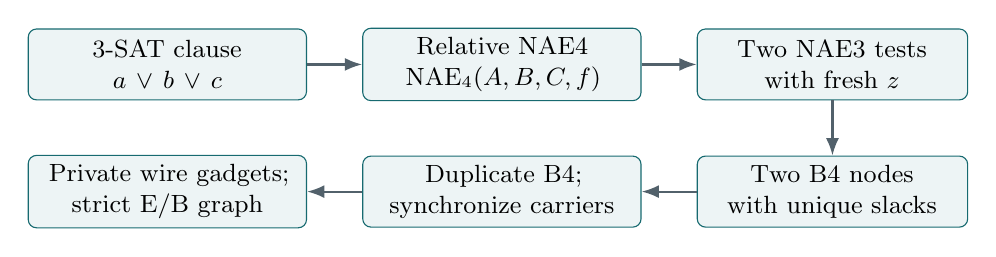
\begin{tikzpicture}[node distance=5mm and 7mm]
 \node[process,text width=33mm] (cnf) {3-SAT clause\\$a\lor b\lor c$};
 \node[process,right=of cnf,text width=33mm] (nae) {Relative NAE4\\$\NAE_4(A,B,C,f)$};
 \node[process,right=of nae,text width=32mm] (split) {Two NAE3 tests\\with fresh $z$};
 \draw[arrow] (cnf)--(nae);\draw[arrow] (nae)--(split);
 \node[process,below=7mm of split,text width=32mm] (bal) {Two B4 nodes\\with unique slacks};
 \node[process,left=of bal,text width=33mm] (eq) {Duplicate B4;\\synchronize carriers};
 \node[process,left=of eq,text width=33mm] (wire) {Private wire gadgets;\\strict E/B graph};
 \draw[arrow] (split)--(bal);\draw[arrow] (bal)--(eq);\draw[arrow] (eq)--(wire);
\end{tikzpicture}
\caption{Exact compilation chain. Every arrow is a constructive existential equivalence, not a decision oracle. The common anchor preserves both orientations.}
\label{fig:compiler}
\end{figure}

\begin{corollary}\label{cor:pnp}
\(\EB\in\mathrm P\) if and only if \(\mathrm P=\mathrm{NP}\). Its complement on valid encodings is coNP-complete under polynomial many-one reductions (or include invalid encodings consistently in the complement language).
\end{corollary}
The construction does not establish a lower bound for the time required by any solver. It also does not preserve arbitrary counts: the relative anchor and auxiliary choices can produce multiple lifts of one source model. Counting, projected counting and decision are different tasks. For longer CNF clauses the pinned benchmark compiler first uses the usual existential 3-CNF chain, for a clause of length $k\ge4$, use $k-3$ fresh auxiliaries: $(a_1\lor a_2\lor t_1)$, the clauses $(\neg t_j\lor a_{j+2}\lor t_{j+1})$ for $1\le j\le k-4$, and $(\neg t_{k-3}\lor a_{k-1}\lor a_k)$. This chain is satisfiable in the auxiliary variables exactly when at least one original literal is true; no claim of parsimonious reduction is needed.

\section{Canonical signed-equality quotient}\label{sec:quotient}
The first solver step is exact normalization of the native source, before branching or introducing a more costly representation. This section specifies a deterministic normal form for the equality and transport fragment; it is not a complete normal form for arbitrary semantic equivalence.

\subsection{Extract and contract parity-connected classes}
Construct a graph \(H_I\) whose vertices are original port IDs. Insert every original signed transport \((p,q,s)\). At each E vertex insert three zero-signed links from its port 0 to its remaining ports. Every link in this graph is an equation of the form \(x_p\oplus x_q=s\).
\begin{theorem}[Exact equality quotient]\label{thm:quotient}
In polynomial time, either exhibit a closed walk in \(H_I\) with odd XOR of signs, certifying \(\UNSAT\), or partition the ports into connected classes \(C_1,\ldots,C_k\) with representative \(r_i=\min C_i\) and offsets \(\sigma_p\in\bits\) satisfying
\begin{equation}\label{eq:quotient}
 x_p=y_{c(p)}\oplus\sigma_p,\qquad \sigma_{r_i}=0.
\end{equation}
Here \(c(p)\) is the class index and \(y_i=x_{r_i}\). Every assignment to the \(k\) quotient bits satisfies the complete original equality/transport subsystem through \eqref{eq:quotient}, and every original assignment satisfying that subsystem decodes uniquely to such a quotient assignment.
\end{theorem}
\begin{proof}
Visit each connected component, choosing its minimum port ID as root. Set root offset zero and propagate \(\sigma_q=\sigma_p\oplus s\) on every link. Inconsistency on a visited edge supplies a closed walk from the two tree paths and that edge; XORing the equations along it gives \(0=1\). Otherwise every edge relation is satisfied by the propagated offsets. All original solutions obey the path equations and hence have the form \eqref{eq:quotient}. Conversely the common class bit cancels in each edge equation, establishing exactness. A graph traversal with sorted roots and a deterministic adjacency order, or parity union-find with canonical minimum-root postprocessing, constructs the class map and a replayable spanning forest. All traversals, original IDs and verification are polynomially bounded in the explicit input length.
\end{proof}
The root order and class numbering depend on the original port IDs, not on the order in which solver tracks discover deductions. This permits independently computed equivalent equality quotients on the same source to be reconciled syntactically. Retain the original-edge and E-vertex provenance for every forest link, and the full map from original ports to class/offset pairs. The map is necessary for witness lifting, conditional guard translation, and verifying all later deductions.

\subsection{Preserve exact occupancy, not parity alone}
For each B vertex \(v\), let \(n^0_{vi}\) and \(n^1_{vi}\) be the number of its four ports in class \(i\) with offset 0 and 1, respectively. Define
\begin{equation}\label{eq:weighted}
 a_{vi}=n^0_{vi}-n^1_{vi},\qquad
 b_v=2-\sum_i n^1_{vi}.
\end{equation}
Since \(y\oplus1=1-y\) for a bit, the original balance condition is exactly the integer equation
\begin{equation}\label{eq:weightedrow}
 \sum_i a_{vi}y_i=b_v,\qquad y_i\in\bits.
\end{equation}
It involves at most four distinct quotient variables, with coefficients between \(-4\) and 4. This retains repeated ports and opposite signs correctly; a zero net coefficient cancels only its algebraic contribution, not its original provenance.

\begin{example}[Cancellation and forced information]
If a B vertex has port expressions \((y,1-y,z,w)\), its exact normalized equation is \(z+w=1\), a complementary pair. If the expressions are \((y,y,z,w)\), its equation is \(2y+z+w=2\). The only legal triples \((y,z,w)\) are \((0,1,1)\) and \((1,0,0)\); the relation is affine after exact local table inspection. Simply taking the original balance modulo two would yield \(z=w\) and lose the link to \(y\). These examples motivate repeated exact local inspection after equality contraction.
\end{example}

For a deterministic syntactic row key, collect equal class IDs, delete zero coefficients, sort nonzero coefficients by class representative, and store the right-hand side. A zero row is either a tautology or an immediate contradiction. For a nonzero row, the gcd of its coefficients must divide its right-hand side; otherwise reject with a divisibility certificate. Divide by the gcd when allowed and choose a positive first coefficient by multiplying the row by \(-1\) if necessary. Identical normalized rows can share one constraint record with a list of original owners. This is a sound exact row normalization and does not purport to recognize all equivalent Boolean relations.

\begin{proposition}[Exact quotient and reconstruction]\label{prop:exact}
If equality normalization does not reject, the Boolean system of all rows \eqref{eq:weightedrow} is feasible if and only if the original network is feasible. The solution maps in \eqref{eq:quotient} establish a bijection between its full quotient assignments and the original port witnesses, before any optional symmetry fixing or variable elimination.
\end{proposition}
\begin{proof}
Theorem~\ref{thm:quotient} establishes a bijection for equality and transport. Under that substitution every B condition is exactly \eqref{eq:weightedrow}. Intersection over all B owners therefore preserves precisely the same assignments. Retaining every class bit, including any free class, is essential for the stated bijection.
\end{proof}

\section{Certified closure and restricted terminals}\label{sec:closure}
\subsection{Unconditional forced-information closure}
Initialize each quotient variable's domain to \(\bits\), except for authenticated guarded restrictions. For each normalized balance row, enumerate its at most \(2^4=16\) local assignments consistent with current domains and any locally projected certified equations. Store the exact allowed words. If no word remains, reject with a table certificate. If all words agree on a variable, restrict its domain. If a pair of ports has a constant XOR across every allowed word, add that equality or complementarity to the parity structure. Reapply the quotient, substitute forced bits, and repeat to a fixed point. One may also add affine consequences obtained from the exact local table's affine hull, or sound local binary clauses representing forbidden pairs, provided the full row relation is retained until an exact replacement is established.

For the baseline fixed-scope rule set, each successful round either fixes a bit, merges two distinct equality classes, or adds a previously independent affine equation or previously unrecorded binary clause. On the original quotient coordinates there are at most \(k\) independent affine equations and \(O(k^2)\) distinct binary clauses; fixed bits and equality merges number at most \(O(k)\). Keeping a fixed original-coordinate ledger avoids resetting this count after reindexing. Use deterministic full scans, restarting only after a new ledger entry; terminate if a full scan adds none. Local scans, Gaussian elimination and 2-SAT consistency checks are polynomial per round for this specified closure. This is a polynomial fixed-point computation for the named rules, not a proof of complete forced information. An arbitrary global backbone query is not a permitted free primitive.

For a guard \(G\), a deduction \(D\) from this closure means \(F_I\land G\Rightarrow D\). It can be applied without an additional conditional split within that guard, but must not be broadcast as unconditional on the root unless the implication with no guard has been checked.

\subsection{Affine and binary terminals}
The affine hull of B4 is the even-parity hyperplane in \(\Ftwo^4\). It has eight words rather than six: \(0000\) and \(1111\) are spurious solutions of the parity relaxation. Gaussian elimination thus gives a sound negative test; a consistent parity system does not establish balance feasibility. If every retained relation is \emph{exactly} affine, Gaussian elimination is a complete decision and witness-reconstruction terminal. To check a finite local relation for this property, compute a point and a basis for its translated span, then compare its cardinality with the span size and verify all words lie in that affine space. Exact 2-CNF terminals similarly require a certified representation of the entire remaining relation, rather than only its binary projections. Mixed affine and binary systems do not automatically inherit either terminal's tractability.

\subsection{Pure balance as a prescribed-degree matching problem}
\begin{proposition}[A pure-B terminal]\label{prop:factor}
Strict signed networks containing only B4 vertices reduce in polynomial time to a prescribed-degree subgraph problem, and hence to general-graph perfect matching. Their feasibility is decidable in polynomial time with explicit witness maps.
\end{proposition}
\begin{proof}
Create a graph with each original vertex requiring selected degree two. For each sign-zero edge, add an ordinary edge between its two owners. Selecting that edge sets both corresponding port bits to one; not selecting it sets both to zero. For each sign-one edge, introduce a private intermediate vertex with required degree one and replace the edge by the two half-edges to its original owners. Selecting exactly one half-edge sets exactly one corresponding original port to one. All original required degrees then equal the sums of their port bits. These mappings are exact in both directions.

For completeness, a prescribed-degree instance with graph \(H=(W,L)\), degrees \(d_w\) and target degrees \(f_w\) reduces to perfect matching by the following incidence construction. Reject if some \(f_w\notin[0,d_w]\). Create one incidence node at each end of every edge, join the two incidence nodes of each edge, and add \(d_w-f_w\) local dummy nodes adjacent to all \(d_w\) incidence nodes of \(w\). In any perfect matching the dummy nodes consume exactly \(d_w-f_w\) local incidence nodes. The remaining \(f_w\) incidence nodes must be paired with their counterparts along original edges, so these paired edges give the required subgraph. Conversely a subgraph with the prescribed degrees pairs its selected incidences across edges and matches all remaining local incidences bijectively to dummies. The construction is polynomial in the explicit graph size. General-graph perfect matching is a classical deterministic polynomial-time problem \cite{edmonds1965}. No general mixed E/B matching terminal follows from this pure-B reduction.
\end{proof}
A pure-E network is decided completely by Theorem~\ref{thm:quotient}. These two easy sublanguages are essential adversarial controls: neither large component size nor large numbers of physical port assignments imply large decision complexity.

\subsection{Exact component and separator operations}
Use the quotient factor graph, with one side for variables and the other for exact retained constraints. Disjoint connected components can be solved separately: feasibility of the conjunction is the conjunction of their feasibility; their witness assignments combine on disjoint variables. When two regions share a boundary \(U\), define the exact response relation
\begin{equation}\label{eq:response}
 R_A(u)=1\iff \exists a\ F_A(a,u),\qquad u\in\bits^{\abs U}.
\end{equation}
When the regions have disjoint private variables and all cross-constraints are represented, their composition is the intersection of their responses on \(U\), with witness reconstruction from the matching boundary word. General joins require the actual joint relation, not a Cartesian product of marginals. For example, \(\{00,11\}\) and \(\{01,10\}\) each project onto both bit values at either coordinate, yet have empty joint intersection.

A certified separator of width \(b\) permits an explicit table of at most \(2^b\) words. Standard dynamic programming on a supplied, verified tree decomposition of width \(O(\log N)\) and polynomial size yields polynomial aggregate table work, with full joins and reconstruction charged. Merely listing a logarithmic boundary does not make the private-region extension queries cheap. Discovery of the decomposition and evaluation of all region responses require their own cost proofs. No universal small-width decomposition is assumed.

\subsection{Joint algebraic and geometric channels}
The existing program uses shared-wheel geometry, guarded DAGs, matching/flow, parity syndromes, integer lattices, nonlinear constraints, and exact interface joins as complementary methods \cite{ebdirective,tracks}. Each method is admitted only with a precisely specified recognizer, source-checked transformation, and bounded work under its hypotheses. A useful hybrid changes another method's representation or acquisition cost: for instance, parity contraction can expose an exact matching subproblem, or a verified matching obstruction can provide a cut that reduces an affine guard domain. Running two solvers independently without exchanging a valid dependency is a portfolio, not a hybrid.

A negative-only relaxation is admissible when every original solution projects to a feasible solution of the relaxation. Infeasibility of the relaxation then proves original infeasibility, even if the reverse implication fails. Feasibility of the relaxation only gives \(\UNK\) unless an exact lift is checked. This asymmetric contract is particularly useful for the UNSAT-focused research queue.

\section{The canonical certified state machine}\label{sec:canonical}
\subsection{State, guards and exact transformation semantics}
A live obligation is a record \(Q=(I,G,R,\mu,\mathcal D)\), with immutable original input \(I\), guard predicate \(G\), residual constraint representation \(R\), reconstruction/provenance map \(\mu\), and a dependency set \(\mathcal D\) of verified certificates. The root has no guard and uses the original network. Every non-root guard must be expressed on original variables, or have a checked interpretation via an exact map. A residual may have new coordinates and need not itself be a strict four-regular graph.

A replacement \(R\rightsquigarrow R'\) is \emph{exact} for \(Q\) when it preserves the decision statement
\begin{equation}\label{eq:exactsem}
 \exists x\,[F_I(x)\land G(x)]\quad\Longleftrightarrow\quad\exists y\,R'(y),
\end{equation}
with checked reduction provenance and a constructive, polynomially costed lifting map from a valid \(y\) to an original witness \(x\) satisfying \(G\). For a negative-only replacement, only the forward implication in \eqref{eq:exactsem} is required, and rejection of \(R'\) is the only decision permitted by that implication. Positive lifting must not be inferred from a one-way relaxation.

A branch operation with child guards \(G_1,\ldots,G_t\) requires certified coverage of the parent:
\[
 F_I\land G\ \Rightarrow\ \bigvee_{j=1}^t G_j,
 \qquad F_I\land G_j\ \Rightarrow\ G\quad(1\le j\le t).
\]
The second implication may instead be enforced syntactically by taking every child guard as a conjunction with \(G\). Each child is processed through its own checked residual map. Parent rejection requires rejection of every child, or a stronger checked certificate covering all children. One child witness suffices for feasibility. Counting additionally requires disjointness or correct overlap accounting; decision needs only coverage. Exact component decomposition is a conjunction node, not a branch disjunction node.

\subsection{Cooperative search and contraction sequence}
The baseline canonical procedure is specified in Figure~\ref{fig:pipeline}. Its fixed-point and terminal modules are usable now. The general search for certified productive contractions, and its aggregate cost and coverage, are explicitly open.
\begin{figure}[!htbp]
\centering
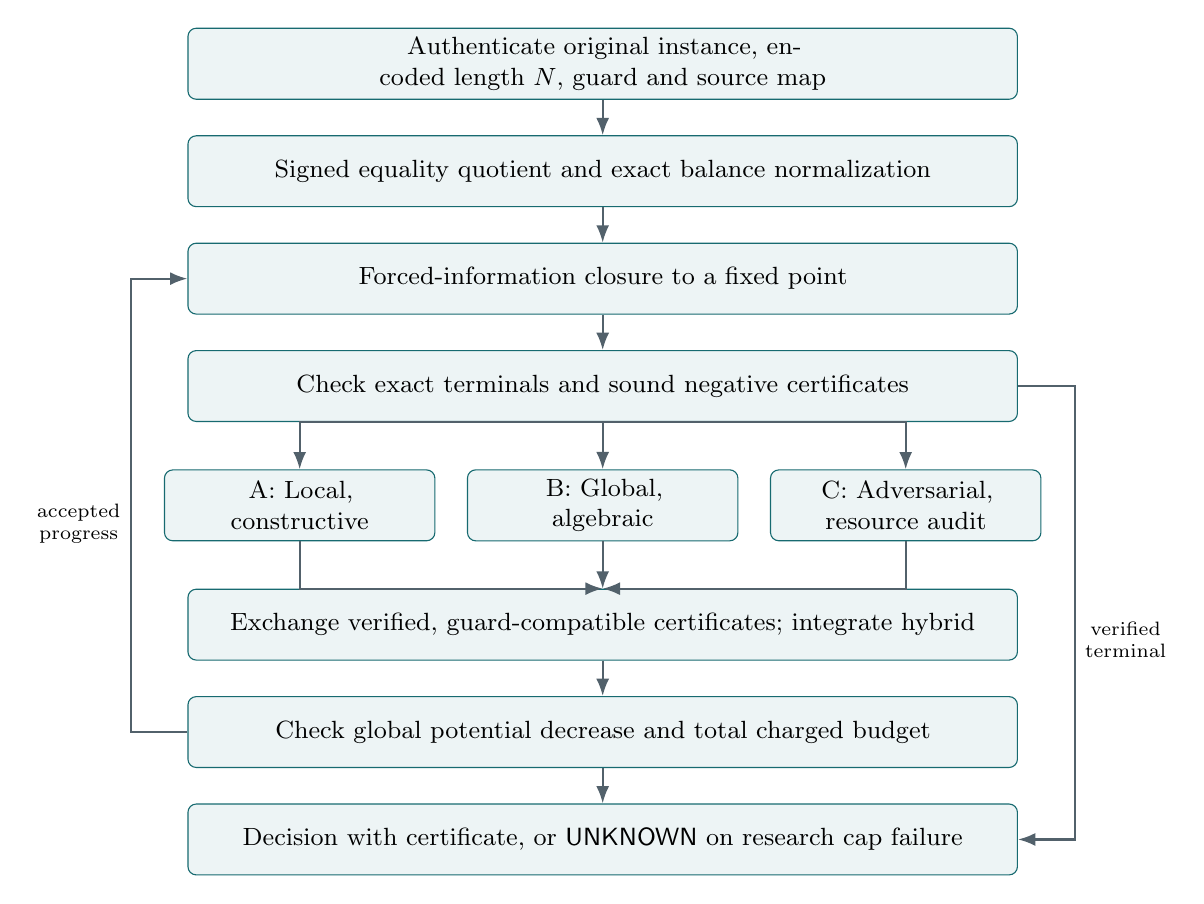
\begin{tikzpicture}[node distance=4.5mm and 4mm]
 \node[process,text width=103mm] (input) {Authenticate original instance, encoded length $N$, guard and source map};
 \node[process,below=of input,text width=103mm] (q) {Signed equality quotient and exact balance normalization};
 \node[process,below=of q,text width=103mm] (cl) {Forced-information closure to a fixed point};
 \node[process,below=of cl,text width=103mm] (term) {Check exact terminals and sound negative certificates};
 \node[process,below=6mm of term,text width=32mm] (b) {B: Global,\\algebraic};
 \node[process,left=of b,text width=32mm] (a) {A: Local,\\constructive};
 \node[process,right=of b,text width=32mm] (c) {C: Adversarial,\\resource audit};
 \node[process,below=6mm of b,text width=103mm] (share) {Exchange verified, guard-compatible certificates; integrate hybrid};
 \node[process,below=of share,text width=103mm] (prog) {Check global potential decrease and total charged budget};
 \node[process,below=of prog,text width=103mm] (done) {Decision with certificate, or $\mathsf{UNKNOWN}$ on research cap failure};
 \draw[arrow] (input)--(q);\draw[arrow] (q)--(cl);\draw[arrow] (cl)--(term);
 \draw[arrow] (term)--(b);\draw[arrow] (term.south) -| (a.north);\draw[arrow] (term.south) -| (c.north);
 \draw[arrow] (b)--(share);\draw[arrow] (a.south)|-(share.north);\draw[arrow] (c.south)|-(share.north);
 \draw[arrow] (share)--(prog);\draw[arrow] (prog)--(done);
 \draw[arrow] (prog.west)--++(-0.72,0)|-node[pos=0.23,left,font=\scriptsize,align=center]{accepted\\progress}(cl.west);
 \draw[arrow] (term.east)--++(0.72,0)|-node[pos=0.28,right,font=\scriptsize,align=center]{verified\\terminal}(done.east);
\end{tikzpicture}
\caption{Canonical cooperative pipeline. The progress gate is a research obligation; returning UNKNOWN is permitted in experiments, not in a proved total decision algorithm.}
\label{fig:pipeline}
\end{figure}

For an unresolved state, each replica begins from the same authenticated source and current guard. First develop and meter its own method. Then exchange only replayed deductions, combine compatible facts with a checked map, and rerun unconditional closure after every accepted import. At stagnation, attempt a genuine alternate representation or hybrid. If a finite budget is exhausted without a valid certificate, record \(\UNK\) and the exact failed rule set, not an asserted contradiction.

A deterministic eventual implementation would specify the schedule and arbitration of candidate modules, canonical tie-breaking, all time caps and the handling of unused credits. A fixed finite module portfolio can be tried in a fixed order, or by deterministic round-robin with exact metering. This gives reproducibility, not coverage. The current multi-agent research execution is an exploratory approximation to that process; independent agents' claims are not automatically a machine-level uniform algorithm.

\subsection{Certificate DAG and verifier contract}
Each certificate node refers to one immutable instance, one guard, one residual and the exact original IDs it affects. The node contains a claim, proof data, an explicit checker, its model, the cited parent certificates and the map needed for subsequent consumers. A verifier checks source identity, guards, dependency acyclicity, local inference, and all referenced input rows or edges. The proof system must admit only explicitly defined sound operations; arbitrary claims such as ``these residuals are equivalent'' cannot be accepted on assertion.

A useful node taxonomy is displayed in Table~\ref{tab:certs}. A shared node is reusable only with identical contextual semantics, or via a verified adapter. Memoizing a node avoids genuine repeated derivation work if it is actually available; validation, retrieval, serialization, reconstruction and every consumer edge still cost resources. A proof DAG's number of nodes alone is not a machine time bound.

\begin{table}[htbp]
\centering\small
\caption{Certificate classes and required checks.}\label{tab:certs}
\begin{tabularx}{\linewidth}{@{}L{0.26\linewidth}YY@{}}
\toprule
Class & Example proof data & Required verification \\
\midrule
Equality or forced bit & Signed forest path; complete local word set & Replay equations or enumerate exact local scope \\
Affine contradiction & Original row combination yielding $0=1$ & Verify every row's source implication and arithmetic \\
Matching/flow obstruction & Exact recognizer and dual or matching certificate & Check graph adapter, demands, scope and obstruction \\
Exact contraction & Regional response plus reverse map & Verify equivalence and reconstructability \\
Guarded rejection & Derivation under retained guard & Check guard, source dependencies and rejection \\
Branch join & All child certificates and coverage proof & Verify exhaustive coverage and every child rejection \\
Potential decrease & Before/after state, credit ledger & Check all unresolved children, budgets and strict decrease \\
\bottomrule
\end{tabularx}
\end{table}

\section{Universal aggregate contraction}\label{sec:potential}
\subsection{The load-bearing theorem}
The original research target is to establish the following proposition. The formulation explicitly rules out counting the smallest child only, restarting budgets on residuals, or assigning a small bit length to a numerically exponential potential. It extends the repository directive \cite{ebdirective} without asserting its conclusion.
\begin{obligation}[Universal certified aggregate contraction]\label{obl:universal}
Find one uniform deterministic algorithm \(A\), fixed polynomials \(p,q,r\), and a nonnegative integer-valued, efficiently evaluable potential \(\Phi_N\) on the complete live state \(S\), satisfying the following conditions for every valid input of original encoded bit length \(N\).
\begin{enumerate}
 \item[\textnormal{(U1)}] Polynomial-time initialization yields \(S_0\) with \(0\le\Phi_N(S_0)\le p(N)\). The state includes all unresolved obligations, contextual maps, proof dependencies, and any credits needed to pay for neutral steps or deferred work.
 \item[\textnormal{(U2)}] Every reachable state correctly represents the root decision problem. A terminal state either verifies an original witness or provides a sound refutation or other correct deterministic negative decision. All invalid or failed candidate transformations are rejected without changing the represented problem.
 \item[\textnormal{(U3)}] At every reachable unresolved state, the algorithm, without an uncharged oracle or advice, either terminates correctly or acquires and verifies a valid state \(S'\) with
 \begin{equation}\label{eq:decrease}
 0\le\Phi_N(S')\le\Phi_N(S)-1.
 \end{equation}
 All intermediate work within this macrostep, including failed attempts, alternate replicas, branching, sharing, candidate verification and representation changes, costs at most \(q(N)\) bit operations. A well-founded amortized recurrence may replace the per-step form only with an explicit polynomial initial credit and a proved aggregate bound.
 \item[\textnormal{(U4)}] Every live representation, map, proof-DAG buffer, output and peak bit-space use is bounded by \(r(N)\) on that same execution. Reconstruction and final checking are polynomial in original \(N\). Cumulative live memory is accounted for over all charged steps and across all simultaneous workers.
\end{enumerate}
\end{obligation}

\begin{theorem}[Conditional termination and complexity]\label{thm:conditional}
If Obligation~\ref{obl:universal} holds, then \(\EB\in\mathrm P\) and hence \(\mathrm P=\mathrm{NP}\). With the strict macrostep formulation and polynomial initialization and finalization times \(T_{\mathrm{init}},T_{\mathrm{fin}}\), a valid bound is
\begin{equation}\label{eq:total}
 T(N)\le T_{\mathrm{init}}(N)+(p(N)+1)q(N)+T_{\mathrm{fin}}(N).
\end{equation}
\end{theorem}
\begin{proof}
Each nonterminal macrostep lowers a nonnegative integer by at least one. Thus there are at most \(p(N)\) productive nonterminal transitions, followed by at most one terminal macrostep. Every reachable state must be covered by U3, including a nonterminal state with potential zero; such a state must terminate, since further strict nonnegative descent is impossible. Summing the charged work, initialization and finalization gives \eqref{eq:total}. U2 and U4 establish correctness and verified output within the declared resources. A standard bit-cost RAM implementation with polynomially bounded memory has polynomial simulation overhead on a deterministic multitape Turing machine; alternatively specify the machine directly. The conclusion then follows from Corollary~\ref{cor:pnp}.
\end{proof}
The theorem is a conditional implication, not a proof that U3 holds. The $+1$ pays for the terminal macrostep even if no potential decrease occurs at that step. An unrestricted existential version allowing a correct polynomial decider as a terminal is equivalent to \(\mathrm P=\mathrm{NP}\): if \(\mathrm P=\mathrm{NP}\), a uniform polynomial decider for \(\EB\) already exists. A checked polynomial witness search can be obtained by polynomially many SAT self-reduction queries, with all such queries executed by the hypothetical decider or a proved polynomial equivalent reduction. A demand for certificates in a specific restricted proof system is an additional requirement and need not follow merely from its stated decision complexity. The nontrivial program goal is to establish U3 constructively for explicit verified operations rather than invoke the very decision algorithm being sought.

\subsection{Why aggregate, not local, descent is necessary}
A tempting potential is the number of remaining quotient variables in the current residual. It decreases if an equality class is eliminated. It also decreases along either child of a single-bit split, yet a complete binary splitting tree of depth \(k\) has \(2^k\) leaves. The sum of remaining variable counts over all unresolved children can increase from \(k\) to \(2(k-1)\). Neither local descent nor short branch depth pays for all required branches. A candidate potential must be applied to the entire outstanding obligation state, with true shared subproblems identified and paid for.

For a bounded exponential kernel, the aggregate criterion is quantitative. If \(M(N)\le N^a\) kernels are acquired and each has at most \(b\log_2 N\) independent binary dimensions, explicit enumeration costs at most \(M(N)N^b\) times a polynomial per state. Both constants \(a,b\) must be fixed independently of the input, and the count of kernels, discovery cost, and interactions must be proved, not inferred from individual small kernels. If the number or dimensions of kernels grow beyond the charged bound, the terminal becomes a parameterized or exponential method rather than a universal polynomial one.

\subsection{UNSAT-only research and quantifiers}\label{sec:unsat}
Experiments focus on authenticated NO instances. A sound negative proof routine may legitimately return \(\UNK\) on every YES input and on some NO inputs. A different, stronger statement would suffice for P=NP: there is a single deterministic routine and fixed polynomial \(P_0\) such that for every valid NO instance it rejects within \(P_0(N)\), and it never rejects a valid YES instance. A decider can then run it for the proved cap, reject if it rejects, and accept otherwise. Without the universally proved NO completeness bound, accepting on timeout is unsound. Soundness on YES must still be verified, even when research only investigates NO sources.

For the separation direction the required quantifiers are
\begin{equation}\label{eq:lowerquant}
 \forall M\in\mathcal M_{\mathrm{correct}}\ \forall c\in\mathbb N\ \forall K>0\ \exists I:\quad T_M(I)>K(1+N)^c,
\end{equation}
where \(\mathcal M_{\mathrm{correct}}\) contains all uniform deterministic total deciders of the specified language in the standard model. This rules out every fixed polynomial. A lower bound for resolution, a static interface representation, a prescribed branching DAG, or a finite solver portfolio does not have those quantifiers. Moreover, a per-instance minimum over all correct programs is not a valid worst-case lower-bound method: for a fixed known input a program can special-case its encoding and answer before invoking any general solver on other inputs. The machine must be fixed before selecting its hostile input. The existence of a small explicit representation and the cost of discovering it are likewise distinct.

\section{Resource ledger and mathematical audit}\label{sec:cost}
\subsection{Same-execution accounting}
Let \(T\) denote total charged bit work, \(S_{\max}\) peak live bits, and \(S_t\) live bits at computational step \(t\). For a serial realization define cumulative memory (bit-steps) by
\begin{equation}\label{eq:cm}
 \mathrm{CM}=\sum_{t=0}^{T} S_t\le (T+1)S_{\max}.
\end{equation}
For simultaneous tracks use the sum of physically live stores at each instant, counting an actually shared physical object once and separate copies separately; sum work over all workers including unsuccessful routes. Wall-clock span does not substitute for total work. A deterministic serial schedule provides a valid upper bound if all inter-track communication, simulation and recomputation are charged. If measuring cumulative memory on a different clock, define that clock explicitly and prove its relation to the bit-step model.

\begin{table}[htbp]
\centering\small
\caption{Mandatory charges in original-input units.}\label{tab:cost}
\begin{tabularx}{\linewidth}{@{}L{0.30\linewidth}Y@{}}
\toprule
Stage & Required ledger entries \\
\midrule
Input and authentication & Parsing, validation, hashing, IDs, source map acquisition, reads and index widths \\
Normalization and discovery & Equality quotient, closure, recognizers, parameter selection, failed searches, algebraic bit precision \\
Branching and composition & All child obligations, interface tables, exact joins, sharing and adapter construction \\
Cooperative exchange & Serialization, transmitted bytes, import validation, replay, duplicate attempts, synchronization \\
Storage and reconstruction & All live residuals, maps, caches, DAG nodes and consumers, recomputation, witness lifting, final checking \\
Termination & Fixed bound on potential/credits, total bit work, peak bits, cumulative bit-steps, output length \\
\bottomrule
\end{tabularx}
\end{table}
A conservative proof may upper-bound all of these charges by products and sums of fixed polynomials, provided every relevant stage and candidate invocation is counted. Counts of local scans, arithmetic operations, solver nodes or abstract events are useful diagnostics, but are not interchangeable with bit-time measurements without a conversion theorem. Real-valued attention, massive parallelism, free memory access or an oracle do not constitute a standard-machine model unless their uniform finite-precision implementation and resource overhead are proved.

\subsection{Required falsification gates}
The following audit conditions apply to claims made with this framework. They are not blanket certificates that the universal proof has passed.
\begin{table}[htbp]
\centering\small
\caption{Audit gates for candidate progress and lower-bound lemmas.}\label{tab:gates}
\begin{tabularx}{\linewidth}{@{}L{0.27\linewidth}Y@{}}
\toprule
Gate & Test and status at specification level \\
\midrule
Exact semantics / DISJ & Check guard coverage, join compatibility, shared-map identity and all witness lifts. Exact local modules above are scoped; universal composition remains open. \\
Easy-family controls & Test equality, affine, matching, 2-SAT, bounded width, compact circuits, padding, gauge changes and alternate encodings. A cheap legal bypass falsifies an overstrong compulsory-work claim. \\
Relativization and algebrization & State whether a proposed unrestricted argument relativizes or algebrizes and identify any nonrelativizing step. No unrestricted separation is proved here. \\
Natural proofs & For a circuit-lower-bound route, check the actual constructivity, largeness and usefulness hypotheses. No such claim is needed for the scoped reductions. \\
Simultaneous DTISP & Charge time and space on the same execution; no independent minima or forbidden-region inference without a valid theorem. Universal bound open. \\
Deterministic configurations & Distinguish possible configurations, actually visited configurations and their encoding. Configuration counts alone do not force exponential runtime. \\
\bottomrule
\end{tabularx}
\end{table}
\clearpage
\section{Canonical instance identity and cooperative protocol}\label{sec:protocol}
\subsection{Byte-level identification}
All agents operate on identical initial inputs and coordinate their deductions through the same instance registry \cite{registry,identifiers}. The problem/model identifier is \id{STRICT-EB4-v1}; the original CNF representation is \id{DIMACS-CNF-v1}. An exact instance identifier has the syntax
\begin{center}
\id{<model-id>:sha256:<64 lowercase hexadecimal characters>}.
\end{center}
The digest is SHA-256 of the exact original encoded bytes \cite{nistsha}. A short ID consists of a human-readable alias, an at-sign, and the first twelve hexadecimal digits. For example, the primary joint-compatibility case is
\begin{center}
\id{EB-JOINT-24@e84a0ab6dc6f}.
\end{center}
The full digest, pinned corpus and pinned compiler establish reproducible byte identity for practical purposes. A hash is not a proof of collision impossibility or semantic equivalence. Compare the actual pinned byte streams if ambiguity occurs. A changed edge sign, vertex order, encoding, relabeling or constraint set requires a new instance ID, even if a mathematical equivalence can subsequently be proved. Related instances may exchange deductions only through a verified adapter. A family name, size or seed alone is not an input identity.

For native network bytes use \id{JSON.stringify} of the ordered object \id{\{format,types,edges\}} followed by LF, with no pretty printing or sorting. The separate source map uses its own exact byte fingerprint. Original CNF bytes are used exactly as stored in the corpus. Each track recomputes the full input digest and \(N\) before using any shared certificate; a mismatch blocks import until corrected.

\subsection{Contextual guard, residual and certificate IDs}
Define \(J(a)\) to be UTF-8 bytes of the prescribed compact JSON serialization of \(a\) plus LF, and let \(h(a)=\sha(J(a))\). The root guard ID is \id{EMPTY} and the root residual ID is \id{ROOT}, scoped by the full instance ID \(i\). For a non-root guard, record a versioned syntax \(g\), artifact digest \(d_g\), and compute
\begin{equation}\label{eq:gid}
 d_G=h([\text{\texttt{PNP-GUARD-v1}},i,g,d_g]).
\end{equation}
Its full ID is \id{GUARD-v1:sha256:} followed by \(d_G\). Simple original-port or CNF-variable guards are sorted lists of pairs \([\text{original ID},\text{bit}]\), with no duplicates or conflicting pins. Complex affine or auxiliary guards require a versioned predicate and checked interpretation in original coordinates.

For a transformed residual, record its representation schema \(s_R\), exact artifact digest \(d_R\), and reconstruction/provenance map digest \(d_\mu\). The literal value \id{IDENTITY} is allowed for the map only if original IDs and witness map are unchanged. With the full guard ID \(i_G\), compute
\begin{equation}\label{eq:rid}
 d_{\mathrm{res}}=h([\text{\texttt{PNP-RESIDUAL-v1}},i,i_G,s_R,d_R,d_\mu]).
\end{equation}
The residual ID is \id{RESIDUAL-v1:sha256:} followed by this digest. Certificate IDs use \id{CERT-v1:sha256:} followed by the digest of the exact certificate artifact bytes. The artifact contains its contextual IDs, claim, proof data, source/checker and parent IDs, but excludes its own ID to avoid self-reference. These are the pinned v1 conventions; more elaborate normal forms may be proposed additively, without changing historical identifiers.

\subsection{Broadcast and dependency protocol}
Each verified deduction is broadcast to the shared GitHub issue \href{https://github.com/j15marti/pnp/issues/328}{\#328} promptly, with the record fields shown below. Each agent reads new entries at startup, before importing dependencies, and before publication. Check every incoming proof against the exact input and guard; independent replay is required even if the sender has the same role or used the same program. Unverified ideas are recorded in owned research notes, not as certified facts. New instances and residual artifacts are registered additively, without overwriting source history or unilaterally changing the shared primary queue.
\begin{table}[htbp]
\centering\small
\caption{Minimum certificate broadcast record.}\label{tab:message}
\begin{tabularx}{\linewidth}{@{}L{0.35\linewidth}Y@{}}
\toprule
Field & Content \\
\midrule
\id{problem_id}, \id{instance}, \id{instance_id} & Versioned model, registry alias, full input ID \\
\id{original_N_bits}, \id{source_pin} & Original encoded length, immutable manifest/commit/path \\
\id{guard_id}, \id{residual_id} & Full contextual IDs, or scoped EMPTY/ROOT \\
\id{original_ids} & Affected original vertices, ports, edges, variables or clauses \\
\id{parents} & Verified certificate IDs and broadcast links \\
\id{claim} & Precise quantified assertion with scope and preconditions \\
\id{certificate}, \id{certificate_id} & Exact artifact, checker, discovery/verification costs, precision and full certificate ID \\
\bottomrule
\end{tabularx}
\end{table}

\subsection{Four cooperating workstreams}
The existing research organization assigns complementary specialties to agents without changing the shared mathematical input \cite{tracks,ebdirective}. The four workstreams are local terminals (equality, flow, matching, balance, wheels and regional closure), projection and algebra (parity, orientation, group orbits, interface response and syzygies), model transfer (replay, physical resource costs, alternate algorithms and counterexamples), and proof synthesis (guarded DAGs, global progress and total credit). Every active agent attacks the same two primary native inputs, and each run maintains local, complementary global and adversarial replicas where feasible. Synthesis roles combine only verified dependencies; no agent is presumed to have run just because a message was sent. Schedules are operational coordination, not evidence of parallel complexity.

\section{Shared benchmark corpus and reproducibility}\label{sec:benchmarks}
The pinned corpus \cite{corpus} contains eighteen known UNSAT CNFs across pigeonhole, Tseitin parity, odd-wheel coloring, cyclic three-dimensional matching, equality-chain, one joint-compatibility core, and generated 3-CNF problems. The strict E/B adapter \cite{compiler} deterministically converts these to native networks with explicit reverse provenance. A separate reference checker for the CNF corpus is available \cite{corpuscheck}. The source labels are audit ground truth; they must not be used as free solver answers.

The two common primary cases, in order, are listed in Table~\ref{tab:primary}. The joint core has a verified exhaustive five-triple reference check in its original 24-variable representation; the random 40-variable CNF has a replayed 63-node reference refutation tree with unit-propagation conflict leaves. Those checks authenticate the original NO labels; Theorem~\ref{thm:npc} transfers them to the strict E/B networks. They are not claims of independent exhaustive native search or worst-case hardness. The large native sizes reflect the explicit simplicity/synchronization compiler overhead, which is intentionally removable by exact equality normalization.
\begin{table}[htbp]
\centering\small
\caption{Initial shared native instances, from the pinned registry.}\label{tab:primary}
\begin{tabularx}{\linewidth}{@{}Yrr@{}}
\toprule
Parameter & EB-JOINT-24 & EB-RANDOM-3CNF-40 \\
\midrule
Source variables & 24 & 40 \\
Source clauses & 170 & 184 \\
Native vertices & 18,931 & 17,765 \\
Native edges & 37,862 & 35,530 \\
Native B vertices & 788 & 736 \\
Original native length $N$ (bits) & 5,363,624 & 5,027,816 \\
Reference status & UNSAT & UNSAT \\
\bottomrule
\end{tabularx}
\end{table}

\textbf{Full native digests (SHA-256):}\par
\id{EB-JOINT-24@e84a0ab6dc6f}\par
{\small\id{e84a0ab6dc6f74deb8daeea2ccd41cca90e3d1294411877a813471760897c209}}\par
\id{EB-RANDOM-3CNF-40@8a18e86479df}\par
{\small\id{8a18e86479df916ea5c7fdd760ccd561e4fea3737a94517ab8dc2d28cc7e6bdb}}

Use the native byte lengths, not the smaller CNF sizes, as \(N\) in native-solver experiments. Distinguish native source-only recognition from provenance-assisted decoding. An adapter-generated map is a legitimate paid input or reconstruction tool when declared; it is not automatically available on arbitrary original E/B networks. The pinned setup compiled eight instances and tested local gadgets; the later registry records generation and fingerprinting of all eighteen native inputs. A full independent solve of all eighteen native graphs was not performed at setup \cite{setup,registry,identifiers}.

\subsection{Reproduction commands}
Download the exact pinned \id{benchmarks.json}, \id{compile.js}, and \id{verify.js} from the references. With Node.js in a directory containing those files, run the following commands; \id{shasum} is available on macOS (or use another standard SHA-256 implementation).
\begin{verbatim}
node verify.js benchmarks.json
node compile.js --audit
node compile.js benchmarks.json JOINT-24 joint24
node compile.js benchmarks.json RANDOM-3CNF-40 random40
shasum -a 256 joint24.eb.json random40.eb.json
wc -c joint24.eb.json random40.eb.json
\end{verbatim}
Compare the output fingerprints with the registry, and multiply byte counts by eight. Preserve the exact generated byte streams and source maps; do not reserialize them with a different property order or whitespace. Every subsequent experimental report must include the original instance and residual IDs, pinned code and actual reference checks, scope, budgets, measured or proven work, failures, and raw evidence. The two primary cases remain fixed until a separately authorized common round is published.

\section{Proof spine and unresolved dependencies}\label{sec:spine}
The following dependency chain defines the publication standard for the research objective.
\begin{table}[htbp]
\centering\small
\caption{Current proof spine and status.}\label{tab:status}
\begin{tabularx}{\linewidth}{@{}L{0.30\linewidth}L{0.21\linewidth}Y@{}}
\toprule
Dependency & Status & Scope or remaining requirement \\
\midrule
Strict E/B source & \status{PROVED} & Explicit reduction and verification, Theorem~\ref{thm:npc} \\
Signed equality quotient & \status{PROVED} & Exact source map and contradiction test, Theorem~\ref{thm:quotient} \\
Balance normalization & \status{PROVED} & Exact integer rows and lift, Proposition~\ref{prop:exact} \\
Restricted closure/terminals & \status{PROVED / SCOPED} & Named local rules, pure-B matching and other exact sublanguages \\
Guarded semantic composition & \status{CONDITIONAL} & Valid only for individually certified equivalences, coverage and maps \\
Universal acquisition of a productive operation & \status{OPEN} & Every reachable unresolved state; no assumed oracle \\
Global potential and aggregate budget & \status{OPEN} & Fixed numeric polynomial, all branches and failed work charged \\
Polynomial decision implication & \status{CONDITIONAL} & Theorem~\ref{thm:conditional}, if U1--U4 are established \\
Unrestricted separation & \status{OPEN} & Requires all-decider transfer; scoped obstructions insufficient \\
\bottomrule
\end{tabularx}
\end{table}
The immediate mathematical target is the connecting lemma that any post-closure, nonterminal residual admits a polynomially acquired exact contraction, a certified negative obstruction, or a fully charged guarded decomposition with strict aggregate progress. At present neither a universal list of terminal cases nor a complete progress measure is known. One may refute a candidate potential, refine its domain, combine independent channels, or establish a narrower theorem with an explicit costed adapter. The necessary endpoint is not a favorable empirical trend but a uniform theorem over every valid original input, or a genuine unrestricted lower-bound argument. This document provides the common language and evidence contract for that work.

\clearpage
\appendix
\section{Complete v1 native instance registry (short IDs)}\label{app:registry}
The following entries are from the immutable registry \cite{registry}. Each short ID resolves to a full native SHA-256 digest, source CNF ID, original bit length and source-map fingerprint in the registry. Short IDs are display conveniences; use full identifiers for machine verification. All instances have inherited verified UNSAT labels through the exact adapter.
\begingroup\small
\begin{longtable}{@{}L{0.51\linewidth}rr@{}}
\toprule
Native short ID & Vertices & Native $N$ (bits) \\
\midrule
\endfirsthead
\toprule
Native short ID & Vertices & Native $N$ (bits) \\
\midrule
\endhead
\bottomrule
\endfoot
\id{EB-PHP-4@4324051d6ead} & 7,634 & 2,110,088 \\
\id{EB-PHP-8@1f51ee862c3f} & 57,508 & 17,514,056 \\
\id{EB-PHP-16@eb7856f5df9a} & 435,512 & 144,411,720 \\
\id{EB-TSEITIN-TORUS-3@8434fd49198c} & 13,255 & 3,728,936 \\
\id{EB-TSEITIN-TORUS-5@5c82db67c59f} & 36,839 & 10,899,976 \\
\id{EB-TSEITIN-TORUS-9@aa1b93cadaf4} & 119,383 & 37,314,056 \\
\id{EB-ODD-WHEEL-5@a73d74fa4e74} & 5,137 & 1,390,952 \\
\id{EB-ODD-WHEEL-9@de25362b04df} & 8,965 & 2,493,416 \\
\id{EB-ODD-WHEEL-17@3c81fc7e5f3b} & 16,621 & 4,698,344 \\
\id{EB-CYCLIC-3DM-4@a6159f098362} & 9,185 & 2,556,776 \\
\id{EB-CYCLIC-3DM-8@d52aaa59c117} & 78,749 & 24,311,176 \\
\id{EB-CYCLIC-3DM-16@e81f00c4ed47} & 627,077 & 211,842,600 \\
\id{EB-JOINT-24@e84a0ab6dc6f} & 18,931 & 5,363,624 \\
\id{EB-EQUALITY-CHAIN-8@c079bb42d963} & 1,485 & 371,656 \\
\id{EB-EQUALITY-CHAIN-32@5f1759818e31} & 5,973 & 1,631,720 \\
\id{EB-RANDOM-3CNF-24@4cacafcead1a} & 10,714 & 2,997,128 \\
\id{EB-RANDOM-3CNF-40@8a18e86479df} & 17,765 & 5,027,816 \\
\id{EB-RANDOM-3CNF-60@59484f6ec3f3} & 26,653 & 7,640,456 \\
\end{longtable}
\endgroup
\section{Provenance and review status}
The reduction in Section~\ref{sec:npc} is a self-contained reconstruction of the existing RT01 proof, not an independent formal-kernel build or a claim of research priority. Sections~\ref{sec:quotient}--\ref{sec:cost} give a precise baseline normalization and operational contracts synthesized from the current project specification; the pure-balance matching adapter is justified explicitly. Numerical registry data are taken from the pinned registry, not recomputed in this manuscript-authoring run. The benchmark generator and verification artifacts are available at their immutable commits. No new native solver performance experiment or third-party mathematical review was performed for this document. Author attribution is left at the research-program level pending the project's preferred publication authorship. The universal theorem and the P versus NP question remain open.

\clearpage
\printbibliography[heading=bibintoc,title={References}]
\end{document}
